\documentclass[10pt,a4paper]{article}
\usepackage[utf8]{inputenc}
\usepackage[english]{babel}
\usepackage{amsmath}
\usepackage{amsfonts}
\usepackage{amssymb}
\usepackage{graphicx}
\usepackage[left=4cm,right=4cm,top=4cm,bottom=4cm]{geometry}
\usepackage{natbib}

\renewcommand{\vec}[1]{\mathbf{#1}}

\newcommand{\vx}{\vec{x}}
\newcommand{\vy}{\vec{y}}
\newcommand{\vf}{\vec{f}}
\newcommand{\vsigm}{\boldsymbol{\sigma}}

\newcommand{\Err}{\mathrm{Err}}
\newcommand{\Exp}{\mathrm{E}}
\newcommand{\Var}{\mathrm{Var}}

\newcommand{\avg}[1]{\langle #1 \rangle}

\newcommand{\Wout}{\hat{\mathrm{W}}_{\rm out}}
\newcommand{\Win}{\hat{\mathrm{W}}_{\rm in}}
\newcommand{\Wrec}{\hat{\mathrm{W}}}

\author{Fabian Schubert}

\title{Sequence Prediction in Recurrent Neural Networks with Local Learning Rules}

\begin{document}
\maketitle

\section{Introduction}


How can a dynamical system with states $\vx(t)$ be modified appropriately, such that it can generate an output signal $\vy(t)$ that mimics or predicts some target signal $\vf(t)$?

One variant of this task consists of training $\vx(t)$ to autonomously generate an output $\vy(t)$ that equals $\vf(t)$.\\
The other task, which we shall focus on, includes feeding the signal $\vf(t)$ into the dynamical system which is the supposed to generate an output $\vy(t)$ that correctly predicts $\vf(t+1)$.

Formally, the goal of such a temporal prediction task is to find a function $\vy(\cdot)$
\begin{equation}
\vy(t) = \vy\left( \vf(t),\vf(t-1),\vf(t-2),...\right)
\end{equation}
such that it minimizes an error measure, typically the RMS
\begin{equation}
\Err\left(\vf(t),\vy(t)\right) = \frac{\sqrt{\left| \vf(t) - \vy(t)\right|^2}}{\Var\left[ | \vf|\right]} \; .
\end{equation}

The general idea of how to approach this is to expand the sequence $\left\{ \vf(t-1),\vf(t-2), ...\right\}$ into some high-dimensional feature vector $\vx(t)$ which is then used to predict $\vf(t)$ by a linear model
\begin{equation}
\vy(t) = \Wout \vx(t) = \Wout \vx\left( \vf(t-1),\vf(t-2),...\right) \;
\end{equation}
This expansion has a potentially unbounded amount of parameters, so one takes a recursive approach:
\begin{equation}
\vx(t) = \vx\left(\vx(t-1),\vf(t-1)\right) \;.
\end{equation}
We can further restrict this form to recursive functions that take the form of a discrete-time recurrent network:
\begin{equation}
\vx(t) = \vsigm \left( \Wrec \vx (t-1) + \Win \vf(t-1) \right) \; .
\end{equation}

Recurrent networks for sequence learning have been extensively studied in the field of machine learning \cite{Rumelhart_1988,Elman_1990}. Generally speaking, a recurrent network serves as a reservoir for storing information about the past of an input stream. In classical machine learning approaches, the sequence learning task is a problem of appropriately setting the linear components of the recursive function as well as of the readout to minimize the error.

\section{Backpropagation Through Time}
The idea of the BPTT algorithm is to unfold recurrent causal relations in the network into a feed-forward network structure, which can then be learned with a normal backpropagation algorithm, see Fig. \ref{fig:BPTT}.
\begin{figure}
\centering
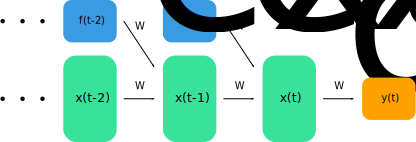
\includegraphics[width=0.6\textwidth]{./figures/backpropagation_through_time.png}
\caption{Illustration of the BPTT algorithm.}
\label{fig:BPTT}
\end{figure}

\subsection{Possible Mechanism of Sequence Learning in the Brain}

Models of error-driven sequence learning have been studied quite extensively, including simple recurrent networks \cite{Elman_1990,Jordan_1989}, as well as the more recent approach of using a Bayesian learning framework to create a generative model of the environment \cite{Friston_2005}. A critical aspect of a predictive framework is that it requires some form of time discretization in order to clearly separate ``future" states or inputs to be predicted from current states. It has been argued that alpha rhythm arising from thalamic neurons might define the pace of such a perceptual and predictive discretization \cite{OReilly_2014}.

Since predictive learning has to be error-driven in some sense, it requires a plasticity mechanism reflecting this requirement. We propose dendritic coincidence detection, gating synaptic plasticity for this purpose. It has been shown that distally evoked dendritic potentials can control plasticity at other synapses \cite{Clopath_Bono_2017}, which fits to the results of the simulations we performed for a single neuron based on a model proposed by Shai et al. \cite{Shai_2015}.

\section{Echo-State Networks}

More recently, so-called echo-state networks have been used in sequence learning \cite{Jaeger_2010}. Instead of training the input, recurrent and output weights, only the readout weights are trained in this framework. A recurrent neural network is randomly created and remains unchanged during training. It needs to contain a large number of nodes ($\sim 10^2 - 10^3$), have a random connectivity structure and must be sparse. The ``echo state property" states that the effect of external input on the internal state should vanish gradually over time.

This architecture is more biologically plausible, since the details of the reservoir are not important, and access to the error is only required for the readout units. Still, the readout needs access to the input signal for comparison, and it is not clear how this could be implemented biologically. Furthermore, readout weights are usually trained via gradient descent of the error, which is not biologically motivated. Ideally, we would like to use an Hebbian type learning rule to learn the readout, while providing some direct access to the input signal to predict.

\section{Dendritic Computation for Sequence Prediction}

Shai et al. proposed a phenomenological model describing neural activity as a function of basal and distal synaptic input in pyramidal neurons \cite{Shai_2015}, see Fig. \ref{fig:Shai_prox_dist}.
\begin{figure}
\centering
\includegraphics[width=0.3\textwidth]{./figures/shai_phen_model.png}
\caption{Firing rate as a function of distal and proximal input of the rate model proposed in \cite{Shai_2015}.}
\label{fig:Shai_prox_dist}
\end{figure}
We further simplified this model to the following form:
\begin{align}
x\left(I_p,I_d\right) &= \sigma\left(I_p-\theta_{p1}\right) \sigma\left(I_d-\theta_d\right)\ +\alpha\sigma\left(I_p-\theta_{p0}\right)\sigma\left(-\left(I_d-\theta_d\right)\right) \label{eq:simpl_prox_dist} \\
\sigma\left(x\right) &= \frac{1}{1+\exp(-g\cdot x)} \label{eq:sigmoidal}
\end{align}
See Fig. \ref{fig:simpl_prox_dist} for a visualization of the relevant parameters.

\begin{figure}
\centering
\includegraphics[width=0.6\textwidth]{./figures/plot_comp_mod_marks.png}
\caption{Output firing rate as a function of proximal and distal input as given by \eqref{eq:simpl_prox_dist}}
\label{fig:simpl_prox_dist}
\end{figure}

We expected the nonlinearity of the neuronal output to be selective for correlated proximal and distal input, such that a Hebbian learning rule allows the neuron to be selective to synaptic input generating the most coherence between distal and proximal input. We tested this hypothesis with a single neuron using the setup illustrated in Fig. \ref{fig:single_neuron_illustration}. The neuron receives $n=10$ proximal input signals $(x_{p1}(t),...x_{pn}(t)$ and a single distal input signal $x_d (t)$. Proximal inputs were generated by simulating a chaotic random network and recording the activity of a randomly chosen unit. Each simulation run corresponds to a single proximal input signal to prevent possible correlations. The distal input was generated as a linear combination of the proximal input streams. In particular, we chose it to be an exact copy of $x_{p1}(t)$ as the most simple case for initial testing. Proximal weights were subject to Hebbian plasticity and weight normalization. The exact mathematical description of the setup is given in \eqref{eq:single_neur_0} -- \eqref{eq:single_neur_5} and Table \ref{tab:single_neuron_parameters}.

\begin{align}
I_p (t) &= \sum_{k=1}^n w_{pk} (t) x_{pk} (t) \label{eq:single_neur_0} \\
x_d (t) &= \sum_{k=1}^n a_k x_{pk} (t), \; \sum_{k=1}^n a_k = 1 \label{eq:single_neur_1} \\
I_d (t) &= w_d x_d (t) \label{eq:single_neur_2} \\
x(t) &= \sigma\left(I_p-\theta_{p1}\right) \sigma\left(I_d-\theta_d\right)\ +\alpha\sigma\left(I_p-\theta_{p0}\right)\sigma\left(-\left(I_d-\theta_d\right)\right) \label{eq:single_neur_3} \\
\Delta w_{pi} (t) &= \epsilon_w \left(x(t)-\langle x \rangle\right)\left(x_{pi}(t)-\langle x_{pi} \rangle \right) \label{eq:single_neur_4} \\
w_{pi}(t+1) &= w_{p,\rm total} \frac{w_{pi}(t) + \Delta w_{pi}(t)}{\sum_{k=1}^n w_{pk}(t) + \Delta w_{pk}(t)} \label{eq:single_neur_5}
\end{align}

\begin{table}
\centering
\caption{Parameter settings for the setup described in \eqref{eq:single_neur_0} -- \eqref{eq:single_neur_5}.}
\begin{tabular}{|c|c|}
\hline
$w_d$ & $1$ \\
$\theta_{p0}$ & $\langle I_p \rangle$ \\
$\theta_{p1}$ & $0.1\langle I_p \rangle$ \\
$\theta_{d}$ & $1.5\langle I_d \rangle$ \\
$\alpha$ & $0.05$ \\
$g$ & $5$ \\
$\epsilon_w$ & $10^{-3}$ \\
$w_{p,\rm total}$ & $1$ \\
\hline
\end{tabular}
\label{tab:single_neuron_parameters}
\end{table}

\begin{figure}
\centering
\includegraphics[width=6.91cm]{./figures/single_neuron_illustration.png}
\caption{A single neuron receiving multiple proximal inputs and a single distal signal.}
\label{fig:single_neuron_illustration}
\end{figure}

A First result is shown in Fig. \ref{fig:single_neuron_results_1}. The correct proximal weight is chosen such that the proximal total input follows the distal input signal. However, when testing the same setup except for a point-neuron summation of both proximal and distal inputs, the same result could be achieved, as shown in Fig. \ref{fig:single_neuron_results_2}. 

\begin{figure}
\centering
\includegraphics[width=\textwidth]{./figures/single_neuron_results_1.png}
\caption{Weights and input signals before and after Hebbian learning of proximal weights, using nonlinear proximal-distal interaction.}
\label{fig:single_neuron_results_1}
\end{figure}

\begin{figure}
\centering
\includegraphics[width=\textwidth]{./figures/single_neuron_results_2.png}
\caption{Weights and input signals before and after Hebbian learning of proximal weights, using linear proximal-distal summation.}
\label{fig:single_neuron_results_2}
\end{figure}

As a further test, we tripled the standard deviation of the second proximal input, thereby making it preferential for the classic scheme of Hebbian learning combined with linear superposition of inputs. This revealed a difference between the proximal-distal activation function and the point neuron: While the proximal-distal scheme was able to select the proximal input that would maximize correlation between proximal and distal signals, the point neuron selected the principal component of the proximal input, in this case being the second input signal. These results are shown in Fig. \ref{fig:single_neuron_results_3} and \ref{fig:single_neuron_results_4}.

\begin{figure}
\centering
\includegraphics[width=\textwidth]{./figures/single_neuron_results_3.png}
\caption{Same setup as in Fig. \ref{fig:single_neuron_results_2}, but with the signal of the second proximal input channel scaled by a factor of three.}
\label{fig:single_neuron_results_3}
\end{figure}

\begin{figure}
\centering
\includegraphics[width=\textwidth]{./figures/single_neuron_results_4.png}
\caption{Same setup as in Fig. \ref{fig:single_neuron_results_1}, but with the signal of the second proximal input channel scaled by a factor of three.}
\label{fig:single_neuron_results_4}
\end{figure}

\subsection{Analytic Approximation of Weight Dynamics}

Assuming that inputs to \eqref{eq:simpl_prox_dist} practically never reach a region where $\theta_{p1}$ becomes relevant, we remove this threshold, resulting in:
\begin{equation}
x\left(I_p,I_d\right) = \sigma\left(I_d-\theta_d\right)\ + \alpha\sigma\left(I_p-\theta_{p0}\right)\sigma\left(-\left(I_d-\theta_d\right)\right) \; . \label{eq:simpl_further_prox_dist}
\end{equation}
We can set both thresholds to zero without loss of generality by assuming that $\langle I_p \rangle = 0$ and $\langle I_d \rangle = 0$. Furthermore, throughout the following calculations, we shall denote $I_p$ by $p$ and $I_d$ by $d$.

To approximate the weight dynamics, we expand the activation function around the mean input (being zero by assumption) to second order. Non mixed square terms turn out to be zero, yielding
\begin{align}
x\left(p,d\right) &\approx  x_0 + \frac{g}{8} \left[ p \alpha  + d(2-\alpha) - pd \gamma\right] \\
\gamma &\equiv \frac{\alpha g}{2} \; .
\end{align}
Plugging this approximation into \eqref{eq:single_neur_4}, we get
\begin{align}
\Delta w_{pi} &\approx \epsilon_w \left(x_0 + \frac{g}{8} \left[ p \alpha  + d(2-\alpha) - pd \gamma\right] -\langle x_0 + \frac{g}{8} \left[ p \alpha  + d(2-\alpha) - pd \gamma\right] \rangle\right)\left(x_{pi}(t)-\langle x_{pi} \rangle \right) \\
&= \epsilon'_w \left(  \alpha (p - \avg{p}) + (2-\alpha)(d-\avg{d}) - \gamma (pd - \avg{pd})\right)\left(x_{pi}(t)-\langle x_{pi} \rangle \right) \\
\epsilon'_w &\equiv \epsilon_w \frac{g}{8}
\end{align}
Further simplification of this equation leads to
\begin{align}
\Delta w_{pi} &\approx \epsilon'_w \sum_j \left( \alpha C^{xx}_{ij} - \gamma C^{dxx}_{ij}\right)w_{pj} + (2-\alpha) C^{dx}_i \\
C^{xx}_{ij} &\equiv \avg{\left(x_i - \avg{x_i} \right)\left( x_j - \avg{x_j} \right)} \\
C^{dxx}_{ij} &\equiv \avg{\left(d - \avg{d} \right) \left(x_i - \avg{x_i} \right)\left( x_j - \avg{x_j} \right)} \\
C^{dx}_i &\equiv \avg{\left(d - \avg{d} \right) \left(x_i - \avg{x_i} \right)}
\end{align}

For a first comparison between full weight dynamics and approximation, see Fig. \ref{fig:weight_dyn_analytic_comp} (!!Better plot to come!!).

\begin{figure}
\centering
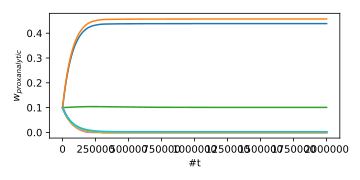
\includegraphics[width=0.7\textwidth]{./figures/weights_analytic_comp.png}
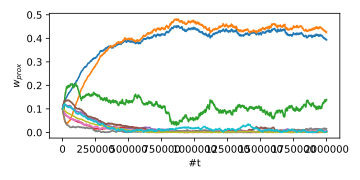
\includegraphics[width=0.7\textwidth]{./figures/weights_full_sim_comp.png}
\caption{Comparison of weight dynamics between analytic approximation and full simulation.}
\label{fig:weight_dyn_analytic_comp}
\end{figure}

\subsection{Adding Plasticity to the Distal Input}

Instead of a single fixed distal input, we used multiple distal inputs with weights $w_{\rm dist, i}$ and applied the same plasticity rule as in \eqref{eq:single_neur_4} and \eqref{eq:single_neur_5}. The input currents were drawn from the same chaotic sequences, where the principle component was aligned with the first input stream, as shown in Fig.~\ref{fig:dist_plast_comp}B (blue trace). The plasticity rule selected this PC from the distal input (Fig.~\ref{fig:dist_plast_comp}C), which allowed the proximal input weights to also align with this component, even though we set the PC of the proximal input to be aligned with the second input stream as a ``distraction, see Fig.~\ref{fig:dist_plast_comp}B,C.

\begin{figure}
\centering
\includegraphics[width=\textwidth]{./figures/dist_plast_comp.png}
\caption{Proximal and distal inputs generated by chaotic sequences ({\bf A},{\bf B}) and the corresponding weight dynamics ({\bf C},{\bf D})}
\label{fig:dist_plast_comp}
\end{figure}


\subsection{Application to a Recurrent Network}

Using the previously described mechanism, we would like to predict an input sequence in a network architecture depicted in Fig. \ref{fig:prox_dist_recurrent}. More precisely, we want the proximal input arriving at the node(s) that were separated in the illustration to be a prediction of the distal input arriving at the same node(s).
\begin{figure}
\centering
\includegraphics[width=0.5\textwidth]{./figures/prox_dist_rnn_illustration.png}
\caption{Combining correlation-sensitive learning with a recurrent reservoir.}
\label{fig:prox_dist_recurrent}
\end{figure}


\subsubsection{Test with a Gradient Descent Rule}
One problem of this setup is the fact that the not yet correlated proximal input to the nodes collecting the proximal input might impede a proper encoding of the distal input signal in the recurrent reservoir. Therefore, we ran a test with the following setup: A single ``hub" node with a proximal-distal activation function was connected to a recurrent reservoir of $N=300$ nodes. The reservoir itself consisted of simple $\rm tanh$ point neurons and a sparse ($p=0.1$) random Gaussian connectivity matrix, drawn from $\mathcal{N}(\mu=0,\sigma=g/\sqrt{pN})$. The connections from the ``hub" node into the recurrent reservoir were fully connected and drawn from $\mathcal{N}(\mu=0,\sigma=1)$. Settings for the proximal-distal activation function as well as for the distal weight were set to the same values as in the previous section. For this test, we used a gradient descent rule for the learning of the proximal weights coming from the reservoir nodes $x_i$, reading
\begin{equation}
\Delta w_i(t) = \epsilon_w \left(I_p(t)-I_d(t)\right) x_i \;.
\end{equation}
The results are shown in Fig. \ref{fig:echo_state_network_pd_act_grad_desc}.

\begin{figure}
\centering
\includegraphics[width=\textwidth]{./figures/echo_state_network_pd_act_grad_desc.png}
\caption{Proximal and distal signal before and after learning, proximal weights during learning}
\label{fig:echo_state_network_pd_act_grad_desc}
\end{figure}

...Still to be done:
\begin{itemize}
\item Hebbian learning rule instead of gradient descent?
\item Use p.-d. activation in the reservoir. Problem: Requires more tuning of parameters (thresholds etc.) to get the ``echo-state property".
\item Is this a good architecture for generalization/multiple layers? Where do feed forward connections go in?
\end{itemize}


\bibliographystyle{unsrt}
\bibliography{/home/fschubert/work/lit_base.bib}
\end{document}